\section{Experimental Evaluation}
\label{sec:evaluation}

We evaluate our Gdev prototype, using the Rodinia
benchmarks~\cite{Che_IISWC09}, GPU-accelerated eCryptfs encrypted
filesystem from KGPU~\cite{Sun_SECURITY11_Poster}, FAST database
search~\cite{Kim_SIGMOD10}, and some dataflow
microbenchmarks from PTask~\cite{Rossbach_SOSP11}.
We disclose that the basic performance of our prototype is practical
even compared to proprietary software, and also demonstrate that Gdev
provides significant benefits for GPU applications in time-sharing
systems.

Our experiments are conducted with the Linux kernel 2.6.38 on NVIDIA
GeForce~GTX~480 graphics card and Intel Core~2~Extreme QX9650 processor.
GPU device programs are compiled by NVCC~\cite{CUDA40} and CPU host
programs are compiled by gcc 4.4.6.

\subsection{Basic Performance}

We first investigate the basic performance of standalone applications achieved
by our Gdev prototype compared to NVIDIA's proprietary driver and
library~\cite{BLOB,CUDA40}, in order to argue that the rest of our
evaluation is practical in the real world. 
To do so, we need to determine what resource parameters maximize
performance for our Gdev prototype.
Figure

\begin{figure}[t]
 \begin{center}
  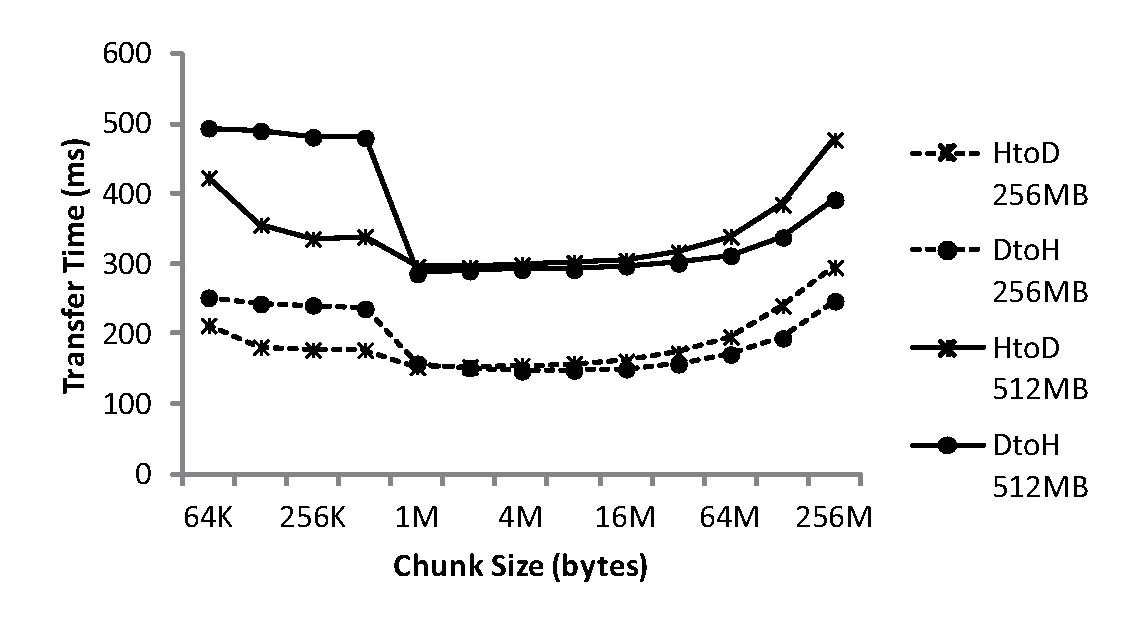
\includegraphics[width=0.95\hsize]{eps/chunk.eps}\\
  \vspace{-1.5em}
  \caption{Impact of the chunk size on DMA throughput.}
  \label{fig:chunk}
 \end{center}
 \begin{center}
  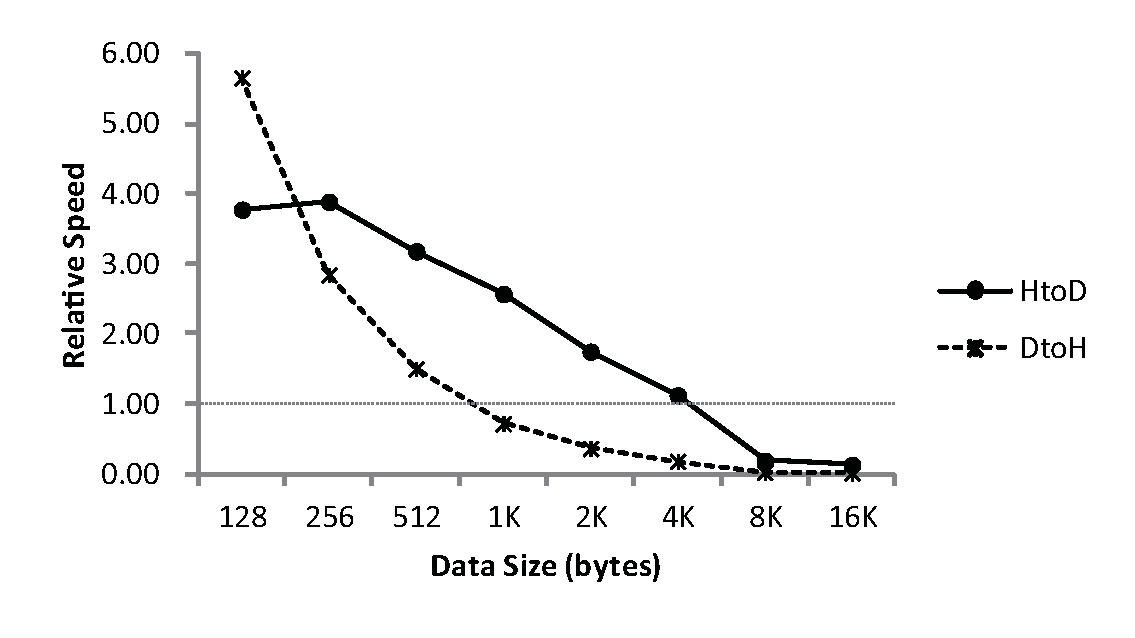
\includegraphics[width=0.95\hsize]{eps/dma.eps}\\
  \vspace{-1.5em}
  \caption{I/O access v.s. DMA.}
  \label{fig:io_access}
 \end{center}
 \begin{center}
  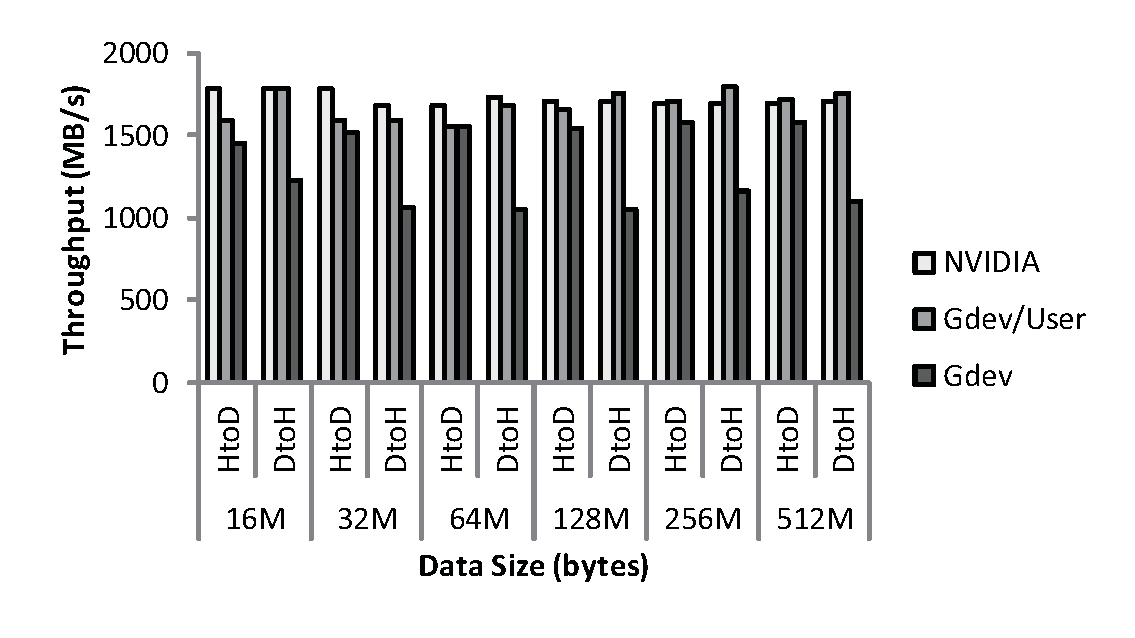
\includegraphics[width=\hsize]{eps/memcpy.eps}\\
  \vspace{-1.5em}
  \caption{Memory-copy performation.}
  \label{fig:memcpy}
 \end{center}
 \vspace{-1.5em}
\end{figure}

\begin{figure}[t]
 \begin{center}
  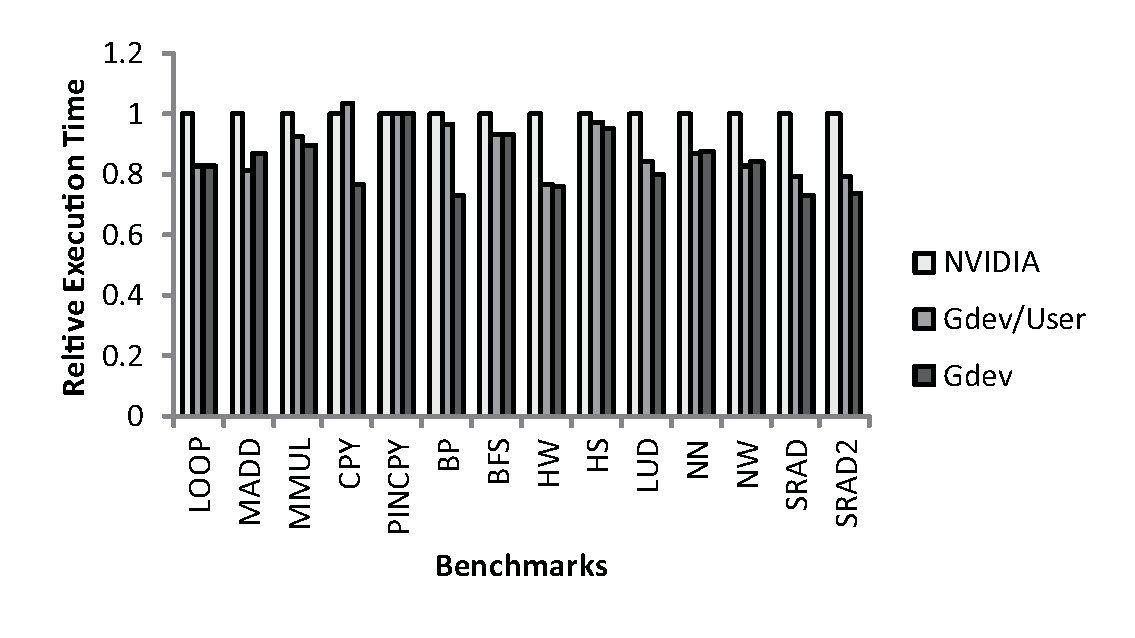
\includegraphics[width=\hsize]{eps/basic_performance.eps}\\
  \vspace{-1.5em}
  \caption{Basic standalone performance.}
  \label{fig:basic_performance}
 \end{center}
 \begin{center}
  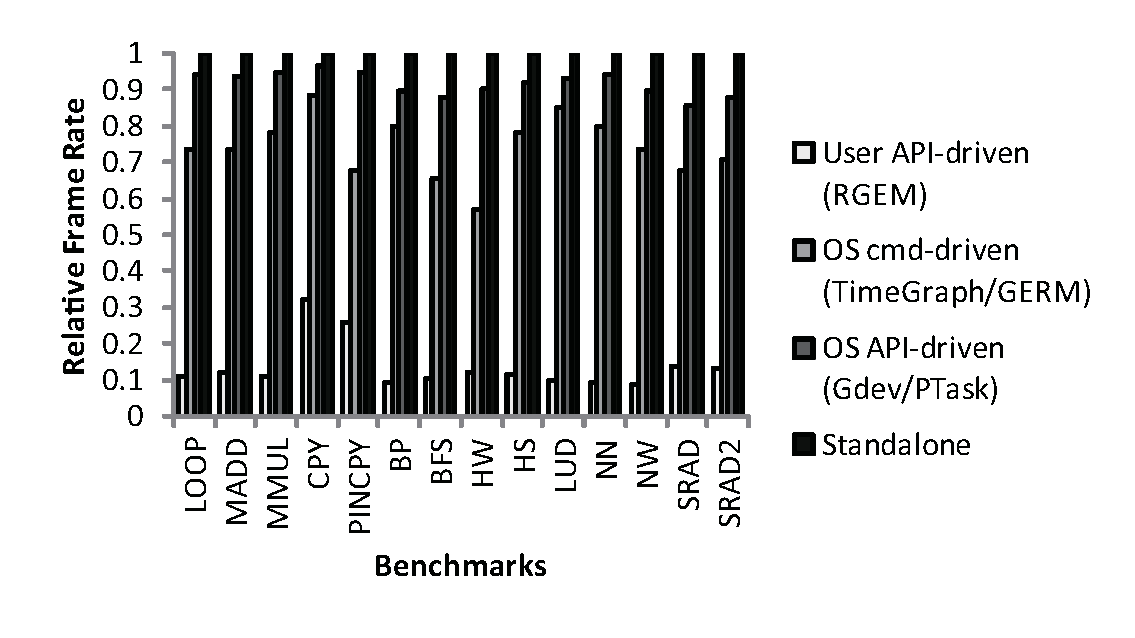
\includegraphics[width=\hsize]{eps/scheduler_overhead.eps}\\
  \vspace{-1.5em}
  \caption{Scheduler overhead under extreme workloads.}
  \label{fig:scheduler_overhead}
 \end{center}
  \vspace{-2em}
\end{figure}

\subsection{Scheduler Overhead}

We next compare overheads of different scheduler designs among Gdev
(API-driven), TimeGraph~\cite{Kato_ATC11} (command-driven), and
RGEM~\cite{Kato_RTSS11} (user-space).

\subsection{OS Applications with GPUs}

\begin{figure}[t]
 \begin{center}
  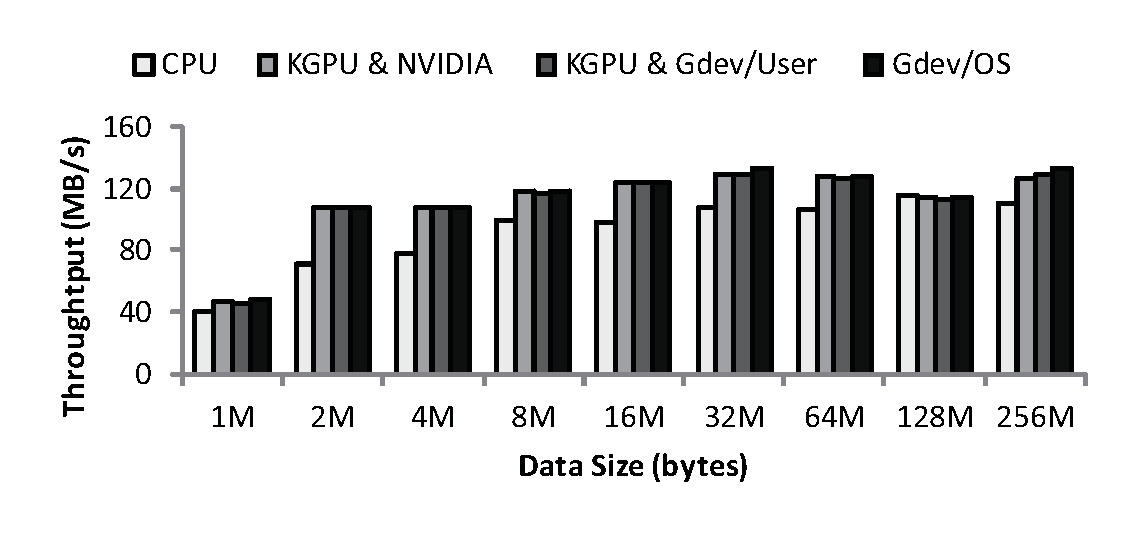
\includegraphics[width=\hsize]{eps/ecryptfs_read.eps}\\
  \vspace{-1.5em}
  \caption{Read throughput of eCryptfs.}
  \label{fig:ecryptfs_read}
 \end{center}
 \begin{center}
  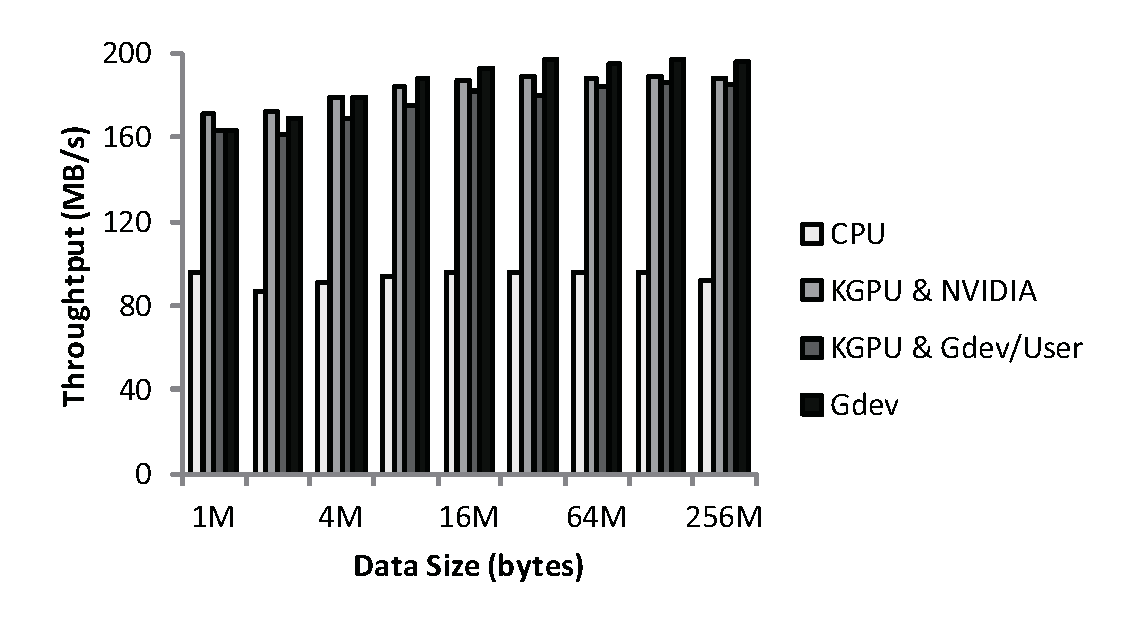
\includegraphics[width=\hsize]{eps/ecryptfs_write.eps}\\
  \vspace{-1.5em}
  \caption{Write throughput of eCryptfs.}
  \label{fig:ecryptfs_write}
 \end{center}
 \begin{center}
  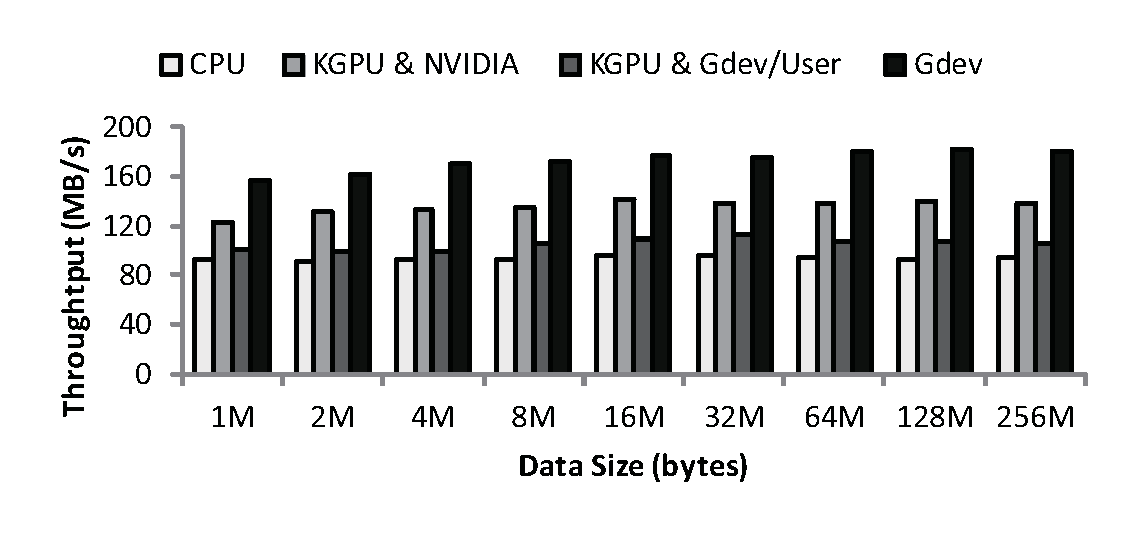
\includegraphics[width=\hsize]{eps/ecryptfs_write_multitask.eps}\\
  \vspace{-1.5em}
  \caption{Write throughput of eCryptfs in mult-tasking.}
  \label{fig:memcpy}
 \end{center}
 \vspace{-2em}
\end{figure}

\subsection{Shared Memory Impact}

\begin{figure}[t]
 \begin{center}
  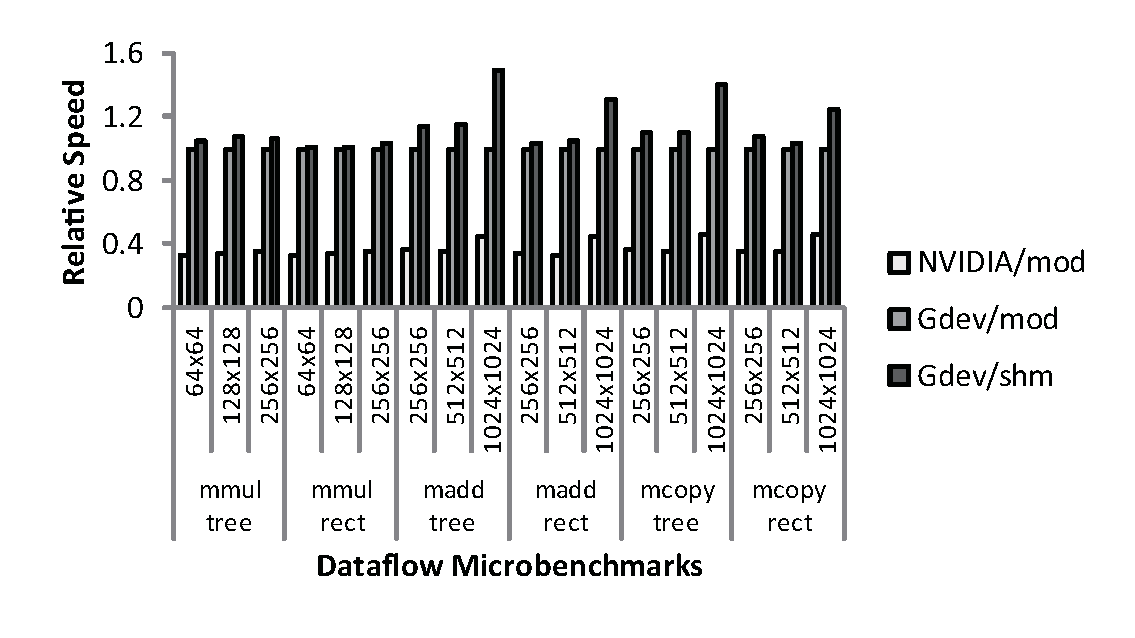
\includegraphics[width=\hsize]{eps/dataflow.eps}\\
  \vspace{-1.5em}
  \caption{Impact of shared memory on dataflow tasks.}
  \label{fig:dataflow}
 \end{center}
 \begin{center}
  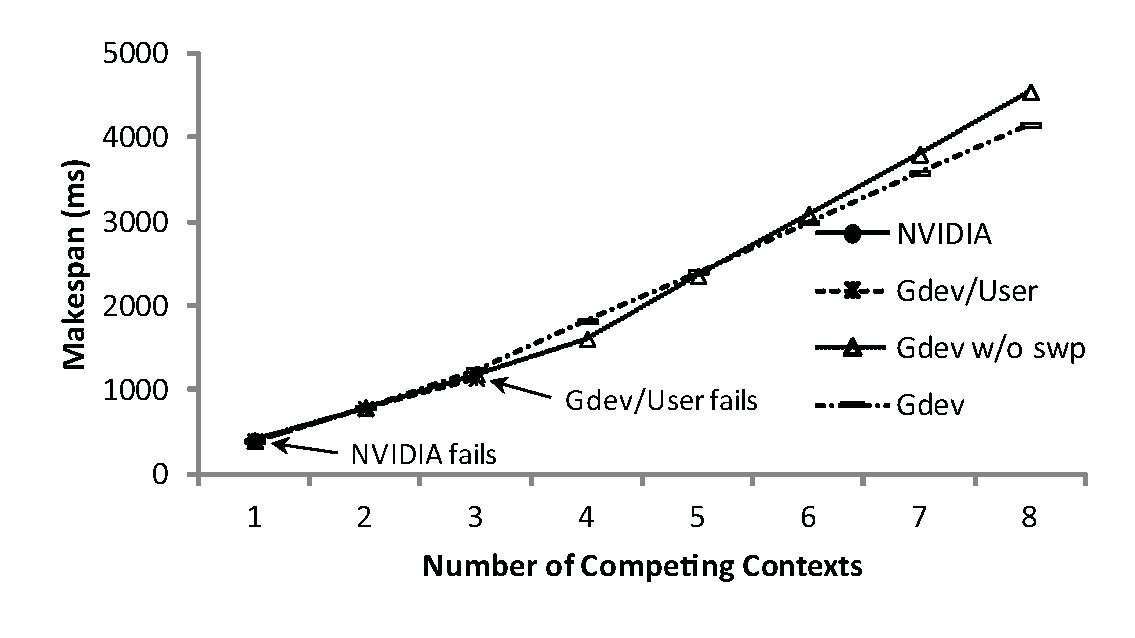
\includegraphics[width=\hsize]{eps/swapping.eps}\\
  \vspace{-1.5em}
  \caption{Impact of swapping latency.}
  \label{fig:swapping}
 \end{center}
  \vspace{-2em}
\end{figure}

\subsection{Virtual GPUs Performance}

\begin{figure*}[t]
 \begin{center}
  \subfigure[FIFO scheduler] {
  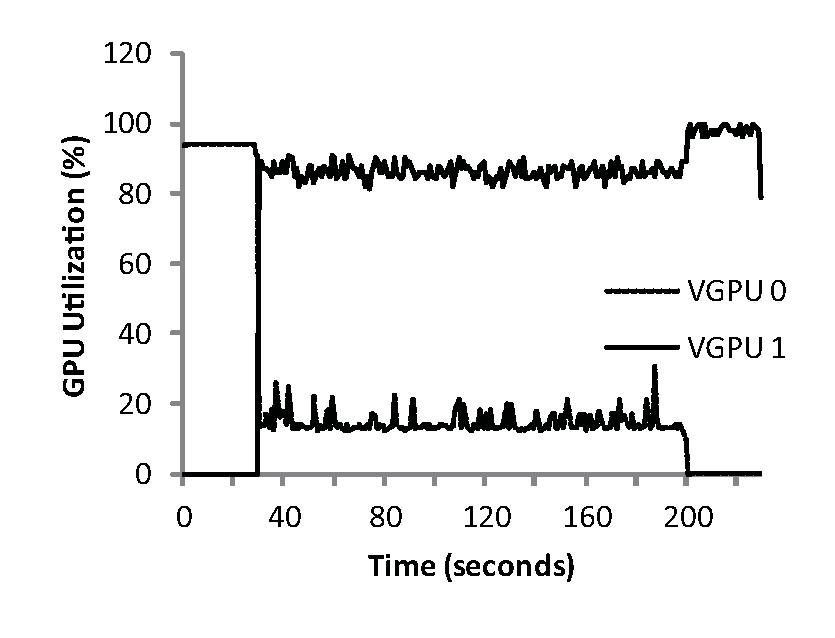
\includegraphics[width=0.319\hsize]{eps/vgpu_2_fifo.eps}
  }
  \subfigure[Credit scheduler] {
  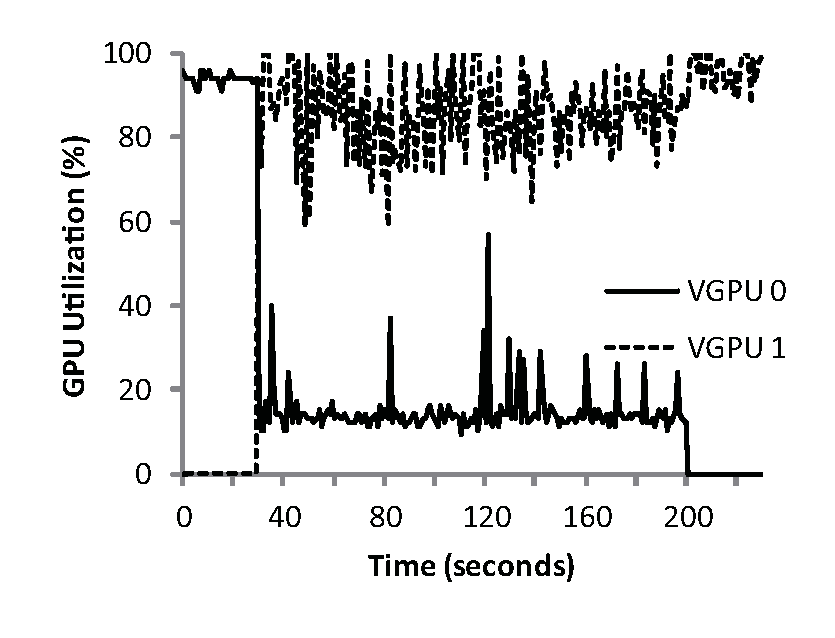
\includegraphics[width=0.319\hsize]{eps/vgpu_2_credit.eps}
  }
  \subfigure[Band scheduler] {
  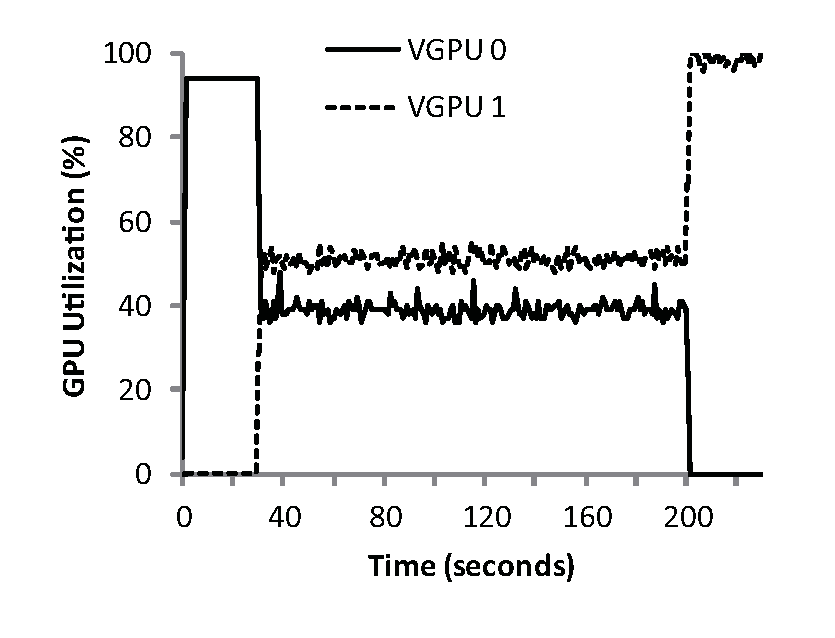
\includegraphics[width=0.319\hsize]{eps/vgpu_2_band.eps}
  }
  \vspace{-1em}
  \caption{Achievable utilization of virtual GPUs.}
  \label{fig:vgpu_2}
  \end{center}
  \vspace{-2em}
\end{figure*}